%%%%%%%%%%%%%%%%%%%%%%%%%%%%%%%%%%%%%%%%%
% Short Sectioned Assignment
% LaTeX Template
% Version 1.0 (5/5/12)
%
% This template has been downloaded from:
% http://www.LaTeXTemplates.com
%
% Original author:
% Frits Wenneker (http://www.howtotex.com)
%
% License:
% CC BY-NC-SA 3.0 (http://creativecommons.org/licenses/by-nc-sa/3.0/)
%
%%%%%%%%%%%%%%%%%%%%%%%%%%%%%%%%%%%%%%%%%

%----------------------------------------------------------------------------------------
%	PACKAGES AND OTHER DOCUMENT CONFIGURATIONS
%----------------------------------------------------------------------------------------

\documentclass[paper=a4, fontsize=11pt]{scrartcl} % A4 paper and 11pt font size

\usepackage[T1]{fontenc} % Use 8-bit encoding that has 256 glyphs
\usepackage{fourier} % Use the Adobe Utopia font for the document - comment this line to return to the LaTeX default
\usepackage[english]{babel} % English language/hyphenation
\usepackage{amsmath,amsfonts,amsthm,amssymb} % Math packages
\usepackage{hyperref}

\usepackage{lipsum} % Used for inserting dummy 'Lorem ipsum' text into the template
\usepackage{graphicx}
\graphicspath{{images/}}
\usepackage{sectsty} % Allows customizing section commands
\allsectionsfont{\centering \normalfont\scshape} % Make all sections centered, the default font and small caps

\usepackage{fancyhdr} % Custom headers and footers
\pagestyle{fancyplain} % Makes all pages in the document conform to the custom headers and footers
\fancyhead{} % No page header - if you want one, create it in the same way as the footers below
\fancyfoot[L]{} % Empty left footer
\fancyfoot[C]{} % Empty center footer
\fancyfoot[R]{\thepage} % Page numbering for right footer
\renewcommand{\headrulewidth}{0pt} % Remove header underlines
\renewcommand{\footrulewidth}{0pt} % Remove footer underlines
\setlength{\headheight}{13.6pt} % Customize the height of the header

\numberwithin{equation}{section} % Number equations within sections (i.e. 1.1, 1.2, 2.1, 2.2 instead of 1, 2, 3, 4)
\numberwithin{figure}{section} % Number figures within sections (i.e. 1.1, 1.2, 2.1, 2.2 instead of 1, 2, 3, 4)
\numberwithin{table}{section} % Number tables within sections (i.e. 1.1, 1.2, 2.1, 2.2 instead of 1, 2, 3, 4)
\makeatletter
\def\@seccntformat#1{%
	\expandafter\ifx\csname c@#1\endcsname\c@section\else
	\csname the#1\endcsname\quad
	\fi}
\makeatother
\makeatletter
\def\@seccntformat#1{%
	\expandafter\ifx\csname c@#1\endcsname\c@subsection\else
	\csname the#1\endcsname\quad
	\fi}
\makeatother
\setlength\parindent{0pt} % Removes all indentation from paragraphs - comment this line for an assignment with lots of text

%----------------------------------------------------------------------------------------
%	TITLE SECTION
%----------------------------------------------------------------------------------------

\newcommand{\horrule}[1]{\rule{\linewidth}{#1}} % Create horizontal rule command with 1 argument of height

\title{	
	\normalfont \normalsize 
	\horrule{0.5pt} \\[0.4cm] % Thin top horizontal rule
	\huge Homework 4 \\ % The assignment title
	\horrule{2pt} \\[0.5cm] % Thick bottom horizontal rule
}

\author{Aaron Gonzales} % Your name

\date{\normalsize\today} % Today's date or a custom date

\begin{document}
	\maketitle
	\section{}
	In this problem we were asked to implement code for logistic regression trained using the Newton-Raphson method. We are also asked to train the data on different training set sizes. Unsurprisingly, it is clear to see in the Accuracy Curve that more training samples yield a higher accuracy on the test data. I was also unsure as to whether or not you wanted us to report on the AUC curve for this problem, I did just in case. The AUC curve in this case closely follows the form of the accuracy curve.  
	 
	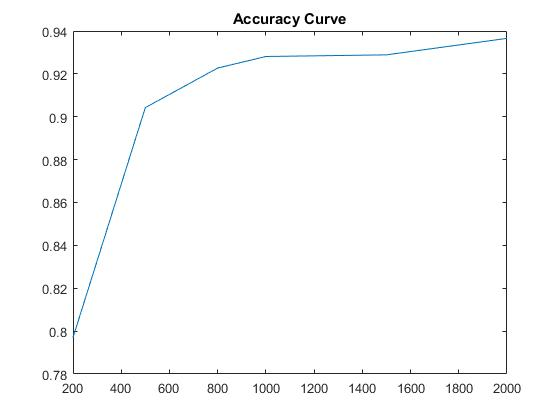
\includegraphics[width=80mm]{acc1}
	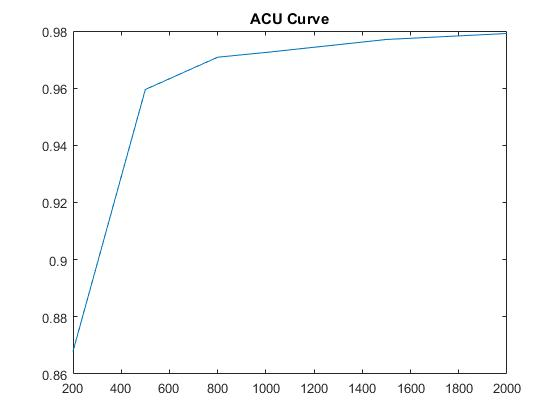
\includegraphics[width=80mm]{auc1}
	\section{}
	In this problem we are asked to perform experiments on sparse logistic regression. We monitor the effects the regularization parameter has in our training, I use 21 values as test regularization parameters, where my reg parameters range from 0 to 1 with 0.05 interval values. While we were not asked to report the accuracy of the experiments I did so out of curiosity and found that the form of the accuracy was quite different than that of the AUC curve. The best regularization parameter for accuracy did not necessarily correspond with the best AUC performance. The AUC curve in this case suggests that the optimal regularization parameter is around 0.1, while the worst is 1. 
	
	
	\quad\quad\quad\quad\quad\quad\quad\quad\quad\quad\quad\quad 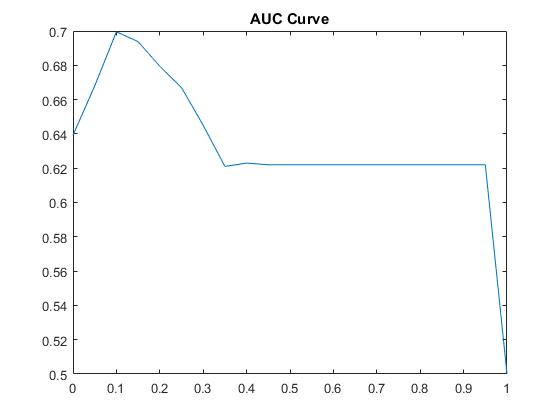
\includegraphics[width=70mm]{auc2}
		
	\href{https://github.com/AaronMG/HW4-ML}{Link to the code available here}.
\end{document}